%\textbf{Intermediate Tile Calorimeter, [PI: De, White]} \
The Intermediate Tile Calorimeter (ITC) was designed to fill the
gaps between the central barrel calorimeter and the extended
barrel calorimeters, and was built at UTA. Figure~\ref{fig:itc_layout_energy} shows a schematic
view of part of the ATLAS calorimeter, showing the
components of the ITC. For particles which originate at the
nominal interaction point, the ITC extends over approximately $0.8
< |\eta| < 1.6$. The region $0.8 < |\eta| < 0.9$ contains 311 mm
thick steel-scintillator stacks, similar in design to standard
Tile Calorimeter submodules. Between $0.9 < |\eta| < 1.0$, the
stacks are 96 mm in the $z$-direction. The combined $0.8 < |\eta|
< 1.0$ region of the ITC is called the plug. In combination with
the support structure for the scintillators, it is called the ITC
submodule. For the forward region, the active elements of the ITC
consist of scintillator only due to space constraints. The
scintillators between $1.0 < |\eta| < 1.2$ are called the gap
scintillators, while those between $1.2 < |\eta| < 1.6$ are called
cryostat scintillators. Some additional scintillators, designated
E4-prime were installed in 2015, covering $1.6 < |\eta| < 1.72$ and
a small sector in $\phi$, in order to explore the possibility of extending
ITC coverage for improved electron and jet measurements.
Together, all these ITC detectors improve the measurement of
total energy in the intermediate region, thereby improving the jet
and \met resolution of ATLAS.

\begin{figure}[htb]
\centering
\subfigure[]{%
      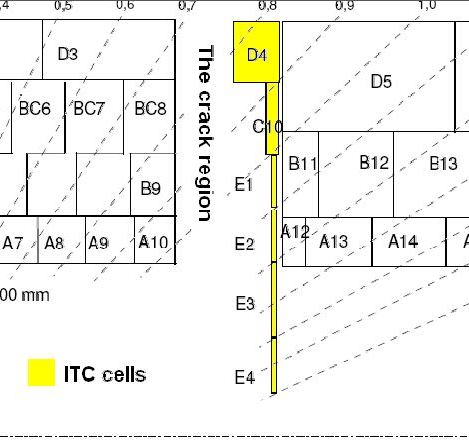
\includegraphics[scale=0.38]{images/ITC_region.jpg}
      \label{fig:itc_layout_energy}
           }
\quad
\subfigure[] {%
       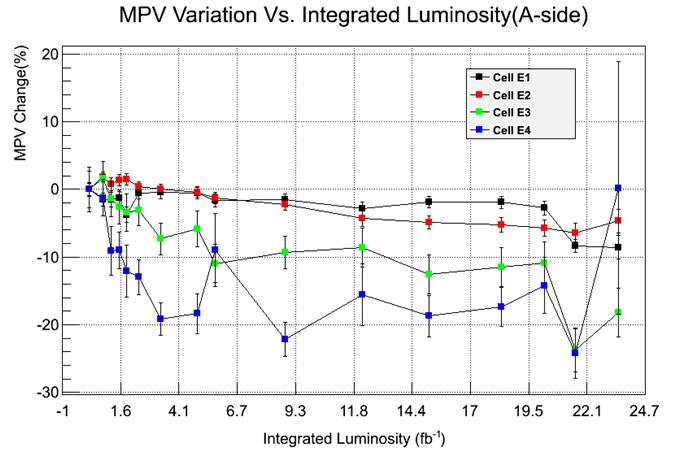
\includegraphics[scale=0.6]{images/itc_MPV_vs_Int_Lumi.jpg}
       \label{fig:Change_vs_Lumi}
           }

\caption{Left - Layout of the Intermediate Tile Calorimeter. Right - Average change for ITC E-modules vs. integrated luminosity.}
\end{figure} 

It is anticipated that the E cell scintillators will need to be replaced in the long 
shutdown in 2019, due to the expected high levels of radiation damage. White, with postdoctoral
associate Park, previously carried out studies of radiation damage using Gaussian plus
Landau fits to the signal distributions for all E-cell channels. This proved to be a very
challenging exercise due to the high degree of variabilty of the signal profiles.
Nevertheless, results were obtained as shown in Figure~\ref{fig:Change_vs_Lumi}. Most of the
decrease in response can be atributed to the downward response of the PMT's due to continual 
exposure to light during the run, as shown by the laser illumination of the photocathodes. 
However, there was a few percent decrease on top of this effect that was attributed to radiation 
damage. This approach to monitoring decreased response has now been replaced with the use of 
minimum bias data plus the laser measurements.
The replacement of the E-cells scintillator affords the opportunity to revisit the $\eta$ and $\phi$ 
segmentation of the cells. In order to determine the best layout for optimization of energy 
resolution in this region, UTA has been working with the Tiblisi group to examine the distributions
of jet energy fractions in the E-cells and the improvement in energy resolution achievable by the
optimal use of the individual E-cell signals. The work at UTA has been carried out by Honors
undergraduate student Niyusha Davachi under White's supervision. As an example, Figure~\ref{fig:E4_Energy_ratios} 
shows the fractional energy contribution for each of the E-cells, for QCD jet events where the jet axis lies in E4,
for three groupings of adjacent $\phi$ cells (3,5, and 7). By studying these fractional energies for jets within all 
the E cell $\eta$ ranges, we will optimize both the use of the deposited energies for jet reconstruction, 
and the propose potential new layout(s) for the E cells. This work is ongoing with the
goal of providing a recommended layout of the new E-cells scintillator in late 2017/18, when the new tiles will 
have to be ordered. 

\begin{figure}[htb]
\centering

      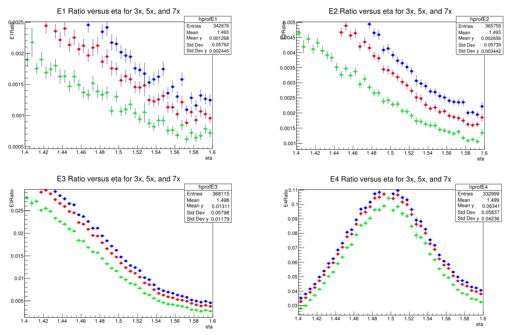
\includegraphics[scale=0.6]{images/E4_Energy_ratios.jpg}
      \label{fig:E4_Energy_ratios}

\caption{Fractional contribution to jet energy by the Ei (i = 1,2,3,4) cells for the case where the jet axis 
lies in the E4 range, $1.4 < |\eta| < 1.6$.}
\end{figure}

While the scintillator replacement is not within the scope of US ATLAS work for Phase I, 
the UTA group has made contributions to the estimation of the expected integrated radiation dose during
Run 2, to the specification and identification of radiation-hard
scintillator, and will be involved in the procurement, installation and testing of the new
tiles. This work will also be included in the qualification tasks for White's new graduate student.

\textbf{ATLAS Tile Calorimeter Timetable of Activities}
Our work on the Tile Calorimeter/ITC will be carried out in collaboration with colleagues
in CERN and Tblisi.

\textbf{2017}
\begin{itemize}[noitemsep,nolistsep]
\item{Complete the study of the optimal use of exisiting E cells for improving jet energy resolution}
\item{Update expected radiation doeses for E cells based on known and projected Run 2 luminosities.}
\item{Study/propose alternative E cells configurations for the 2019 tile replacements}
\item{Continue as a member of the Tile Calorimeter Speakers' Committee.}
\item{Contribute DQ Validator shifts}
\end{itemize}

\textbf{2018}
\begin{itemize}[noitemsep,nolistsep]
\item{Complete plans for ATLAS ITC Tile/Fiber replacements in LS2.}
\item{Investigate the availablity of radiation-hard scintillator for new ITC tiles.}
\item{Prepare (with ATLAS Tile Institutes) tile/fiber assemblies for installation in LS2.}
\item{Graduate student begins time at CERN, with Tile Calorimeter qualification tasks.}
\item{Contribute DQ Validator shifts}
\end{itemize}

\textbf{2019}
\begin{itemize}[noitemsep,nolistsep]
\item{Study effects of radiation on light yield/transmission for dismounted ITC tiles.}
\item{Contribute effort to installation and testing of the new ATLAS ITC E-cells.}
\item{Graduate student returns to UTA.}
\end{itemize}
